\documentclass{beamer}
%Для защит онлайн лучше использовать разрешение 16x9
%\documentclass[aspectratio=169]{beamer}

\input{preamble.tex}

% То, что в квадратных скобках, отображается внизу по центру каждого слайда.
\title[AMO Unit]{Atomic Unit in Vortex GPU}

% То, что в квадратных скобках, отображается в левом нижнем углу.
\institute[SPBU]{}

% То, что в квадратных скобках, отображается в левом нижнем углу.
\author[Shamil Shaehmitov]{Shamil Shaehmitov, SPBU SE}

\begin{document}
{
\setbeamertemplate{footline}{}
% Лого университета или организации, отображается в шапке титульного листа
\begin{frame}
  \includegraphics[width=1.4cm]{pictures/SPbGU_Logo.png}
\vspace{-35pt}
\hspace{-10pt}
\begin{center}
   \begin{tabular}{c}
        \scriptsize{St. Petersburg State University} \\
        \scriptsize{Software Engineering Chair}
    \end{tabular}
\titlepage
\end{center}

\btVFill

\begin{center}
  \vspace{5pt}
  \scriptsize{Saint Petersburg \\
  2026}
  \end{center}

\end{frame}
}



\begin{frame}[fragile]
  \frametitle{Introduction}
  \begin{itemize}
    \item \focus{\href{https://github.com/SparseLinearAlgebra/spla}{Spla}}: sparse-linear-algebra-based graph analysis library that uses OpenCL
    \item Our \focus{goal}: to run Spla on Vortex and conduct experiments
    \item Linear algebra kernels heavily rely on atomic operations
    \begin{itemize}
      \item[\faCheck] Support for atomics has been added in PoCL
      \item[\faFrownO] In the RTL design, support for extension RISC-V A was missing
    \end{itemize}
    \item We have implemented atomic operation support in RTL
    \begin{itemize}
      \item[\faExclamation] Designed to enable experiments on FPGA, not to achieve optimal performance
      \item[\faGears] The implementation is currently under active development
    \end{itemize}
  \end{itemize}
\end{frame}

\begin{frame}
  \frametitle{Memory Lock Arbiters}
  \begin{itemize}
    \item The memory was divided into regions, each of which was assigned an arbiter
    \item The arbiters for global memory are located at the topmost level
    \item When one of the LSUs needs to perform an atomic operation in a region, the arbiter grants permission in a round-robin order
    \item The same arbiters are implemented for local memory if the core has more than one LSU
    \item The number of regions is configurable
  \end{itemize}
\end{frame}

\begin{frame}
  \frametitle{Memory Lock Arbiters}
  \begin{center}
  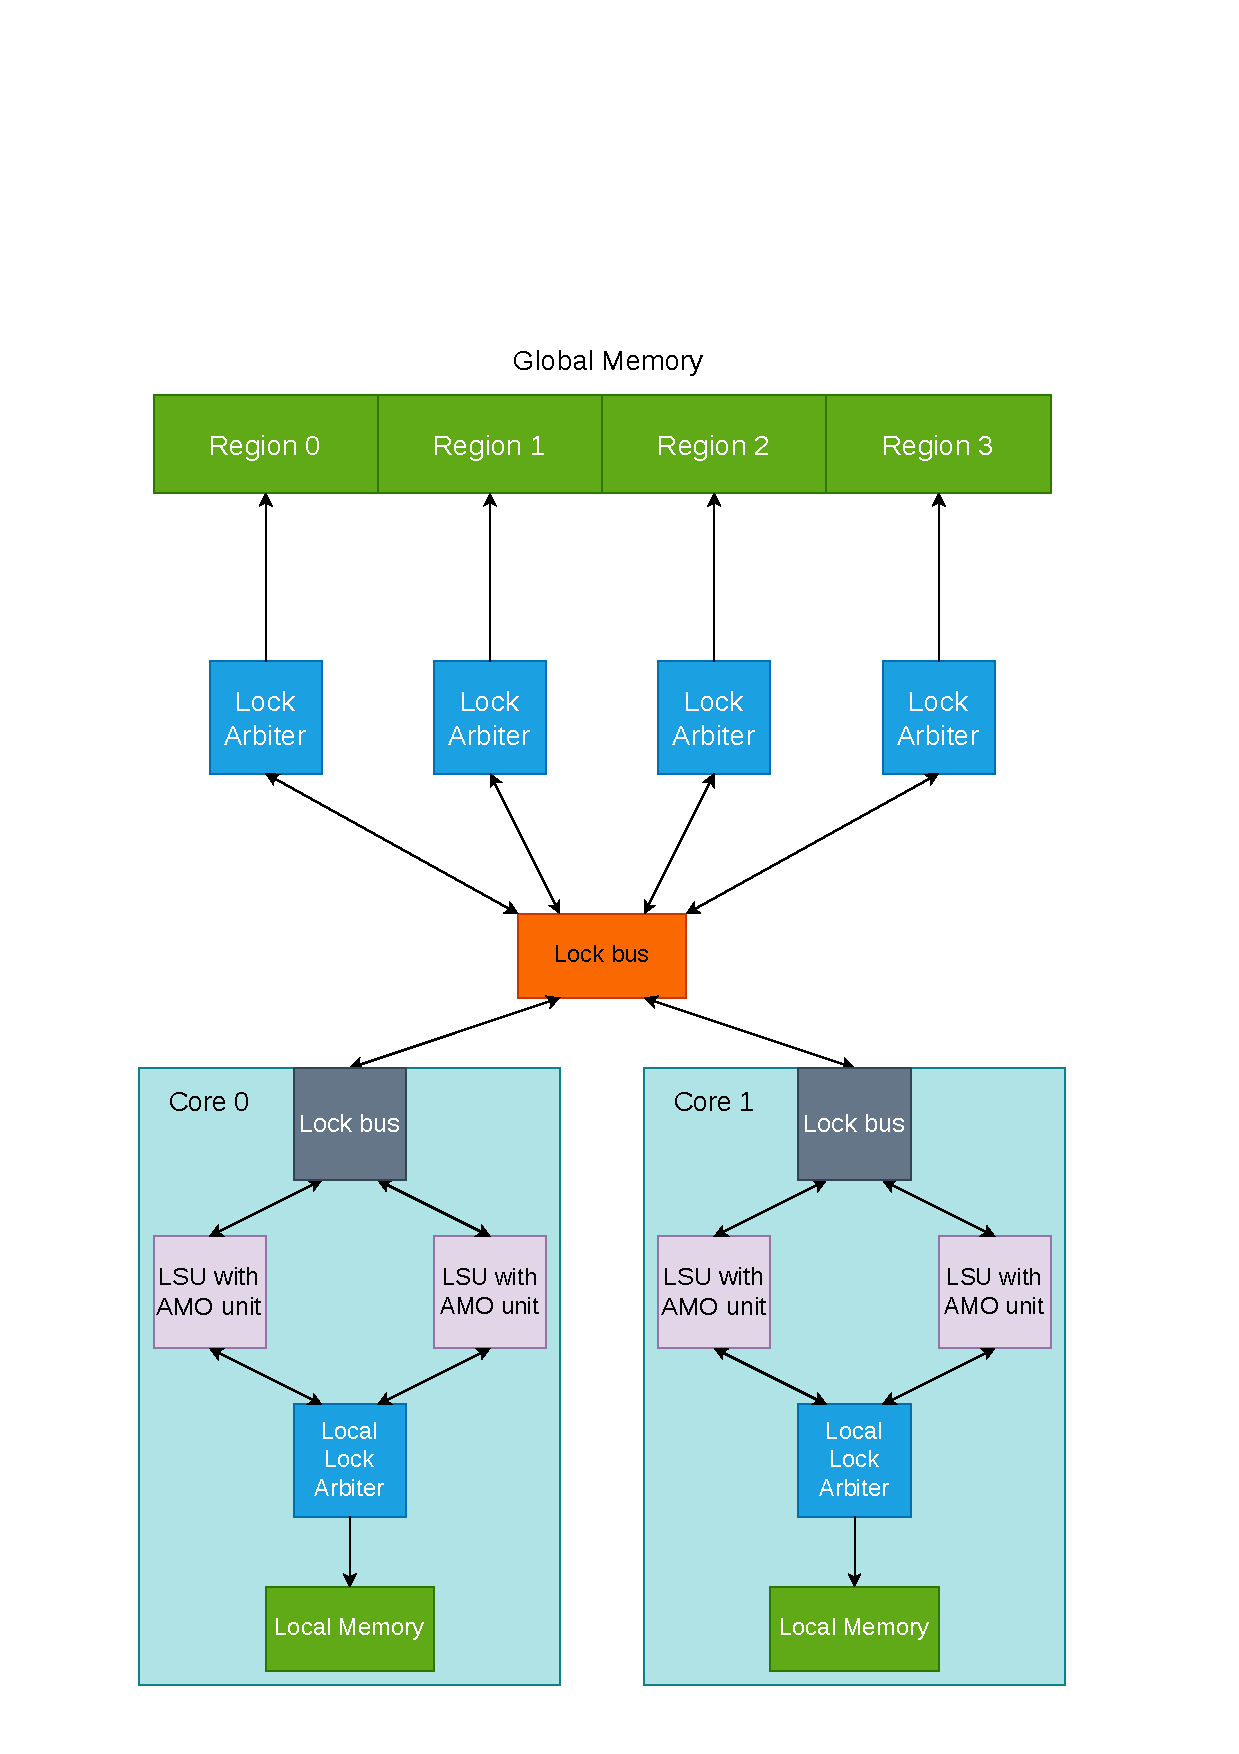
\includegraphics[width=0.45\textwidth]{pictures/amounit.pdf}
  \end{center}
\end{frame}

\begin{frame}
  \frametitle{Atomic Unit}
  \begin{itemize}
    \item Placed in the LSU
    \item The AMO unit is connected to the arbiters via a bus that allows the unit to request a lock and the arbiters to grant it
    \item It is a finite state machine with 9 states
    \item States
    \begin{itemize}
      \item IDLE: waiting for a request
      \item LOCK: waiting for the lock to be granted
      \item DRAIN: waiting for the pipeline to be drained
      \item READREQ: sending a read request
      \item READRSP: waiting for a read response
      \item WRITEREQ: sending a write request
      \item WRITERSP: waiting for a write response
      \item FENCEREQ: sending a dummy read request before lock release
      \item FENCERSP: waiting for a dummy read response
    \end{itemize}
  \end{itemize}
\end{frame}

\begin{frame}
  \frametitle{Optimization 1[WIP]}
  \begin{itemize}
    \item Memory banks are processed sequentially
    \item This makes it possible to complete all operations with fewer lock requests
    \item It also requires entering the FENCE state less often
  \end{itemize}
\end{frame}

\begin{frame}
  \frametitle{Optimization 2[WIP]}
  \begin{itemize}
    \item Skipping read and write operations for consecutive operations to the same address
    \item The read occurs during the first operation
    \item The write occurs during the last operation
  \end{itemize}
\end{frame}

\begin{frame}
  \frametitle{LR/SC instructions}
  \begin{itemize}
    \item LR/SC instructions are implemented using the same atomic unit
    \item The LR instruction is implemented as a read operation with a lock request
    \item The SC instruction is implemented as a write operation with a lock request
    \item Two register arrays of size $WARPS\_PER\_LSU \ast NUM\_THREADS$ are used to track the reservation: reservation address and data
  \end{itemize}
\end{frame}

\begin{frame}
  \frametitle{Conclustion}
  \begin{itemize}
    \item Our implementation
    \begin{itemize}
      \item Atomic Unit: \url{https://github.com/talubik/vortex/tree/amo_unit_rtl}
      \item Atomic operations in PoCL: \url{https://github.com/vortexgpgpu/pocl/commit/70db40e299b7a8e4a7e3897339621030f626bb48}
    \end{itemize}
    \item Future work
    \begin{itemize}
      \item Implement basic improvements
      \item Run Spla in RTL simulation and on FPGA
      \item Compare our atomics with \href{https://github.com/Vaibhav110/Vortex_gpgpu_atomicity/commits/master/}{baseline}
      \item What about \href{https://ieeexplore.ieee.org/document/10764542}{``Atomic Cache: Enabling Efficient Fine-Grained Synchronization with Relaxed Memory Consistency on GPGPUs through In-Cache Atomic Operations''}?
    \end{itemize}
  \end{itemize}
\end{frame}


\begin{frame}
  \frametitle{Other Links}
  Our Pull Requests with various fixes for Vortex:
  \begin{itemize}
    \item CopyBuff operation support: \url{https://github.com/vortexgpgpu/vortex/pull/310}
    \item VX Spawn Fix: \url{https://github.com/vortexgpgpu/vortex/pull/321}
  \end{itemize}
\end{frame}

\end{document}
